% BHU PYQ -- Manually transcribed & error-corrected
% Paper: GLB-502: Igneous Petrology, Mineralogy and Crystallography
% Exam: B.Sc. (Hons.) Semester V Examination, 2022-23

\documentclass[11pt,a4paper]{article}
\usepackage[a4paper,top=2.5cm,bottom=2.5cm,left=2.8cm,right=2.8cm,headheight=14pt]{geometry}
\usepackage{amsmath,amssymb}
\usepackage[T1]{fontenc}
\usepackage[utf8]{inputenc}
\usepackage{lmodern,microtype,fancyhdr,enumitem,hyperref,lastpage,parskip}
\usepackage{tikz}

\hypersetup{colorlinks=true,urlcolor=black,linkcolor=black,
  pdftitle={GLB-502 Igneous Petrology, Mineralogy and Crystallography -- BHU B.Sc. Sem V 2022-23}}
\pagestyle{fancy}\fancyhf{}
\renewcommand{\headrulewidth}{0.4pt}\renewcommand{\footrulewidth}{0.4pt}
\fancyhead[L]{\small   \textit{Banaras Hindu University}}
\fancyhead[R]{\small   \textit{GLB-502: Igneous Petrology, Mineralogy \& Crystallography}}
\fancyfoot[C]{\small Page  \thepage\ of \pageref{LastPage}}


\newlist{parts}{enumerate}{2}
\setlist[parts,1]{label=(\alph*),leftmargin=*,itemsep=5pt,topsep=3pt}

\newlist{subparts}{enumerate}{2}
\setlist[subparts,1]{label=(\roman*),leftmargin=*,itemsep=5pt,topsep=3pt}

\newcommand{\pts}[1]{\hfill   \textit{[#1]}}


\begin{document}

\begin{center}
  {\large\bfseries BANARAS HINDU UNIVERSITY}\\[2pt]
  {\normalsize B.Sc. (Hons.) --- Semester V Examination, 2022-23}\\[6pt]
  \rule{0.8\linewidth}{0.5pt}\\[6pt]
  {\large\bfseries Paper: GLB-502 --- Igneous Petrology, Mineralogy and Crystallography}\\[4pt]
  {\normalsize Time: 3 Hours \hfill Maximum Marks: 70}\\[2pt]
  {\small Ref. No.: 052658}
\end{center}
\rule{\linewidth}{0.4pt}
\smallskip



\noindent   \textit{Instructions: Answer   \textbf{five} questions in all, selecting at least   \textbf{two} questions each from Sections A and B. Section-C is compulsory. All questions carry equal marks.}
\bigskip

\bigskip


\noindent {\large\bfseries SECTION --- A}
\rule{\linewidth}{0.4pt}\smallskip




\noindent   \textbf{Question 1.} Justify the following sentences (if necessary with suitable sketches): \pts{14}

\begin{parts}
  \item The solvus in the orthoclase-albite system is convex upward.
  \item Calc-alkaline rocks are confined to subduction zones.
  \item Pegmatite and aplite have the same mineralogical composition as granite but have different textures.
  \item Fractional crystallization does not affect the path followed by the liquid in eutectic systems.
\end{parts}

\medskip


\noindent   \textbf{Question 2.} Discuss the following two processes using any suitable phase diagram: \pts{14}

\begin{parts}
  \item The formation of resorption texture.
  \item Normal zoning in plagioclase.
\end{parts}

\medskip


\noindent   \textbf{Question 3.} Differentiate between   \textbf{ANY THREE} of the following: \pts{14}

\begin{parts}
  \item Spherulitic growth and variolitic growth
  \item Homogeneous and heterogeneous nucleation
  \item Continuous and discontinuous reaction
  \item Orthocumulate and adcumulate
\end{parts}

\medskip


\noindent   \textbf{Question 4.} Answer the following parts: \pts{14}

\begin{parts}
  \item A geologist working in cratonic terrain wanted to classify the rock types of the terrain, and he noted the following observations for rocks at distant places:
  
  Medium to coarse-grained rocks, dominated by felsic minerals, presence of the following number of minerals after counting many observation grids:
  
\begin{subparts}
    \item Quartz 30; alkali feldspar 60; plagioclase feldspar 10; biotite 07; tourmaline 03.
    \item Quartz 11; alkali feldspar 39; plagioclase feldspar 85; Mica 5.
  \end{subparts}
  Name Rock I and Rock II as per the above description. \pts{5}
  
  \item Draw the IUGS classification diagram for plutonic ultramafic rock types. \pts{5}
  
  \item Describe the Dacite and Granodiorite rock types. \pts{4}
\end{parts}

\bigskip


\noindent {\large\bfseries SECTION --- B}
\rule{\linewidth}{0.4pt}\smallskip




\noindent   \textbf{Question 5.} Write an essay on the mica group of minerals giving the general formula, structure, classification, and paragenesis with neat sketches, where applicable. \pts{14}

\medskip


\noindent   \textbf{Question 6.} Write short notes on   \textbf{ANY TWO} of the following: \pts{14}

\begin{parts}
  \item Classification of feldspars
  \item H-M Symbols (Hermann-Mauguin symbols)
  \item Factors controlling solid solution in minerals
\end{parts}

\medskip


\noindent   \textbf{Question 7.} How do we project any crystal or crystal model from spherical projection to stereographic projection? Describe the details of the stereonet which is used in crystallography and mention various symbols used to describe symmetry operations. Write a step-wise description of plotting $\varphi$ on the stereonet. \pts{14}

\bigskip


\noindent {\large\bfseries SECTION --- C}
\rule{\linewidth}{0.4pt}\smallskip




\noindent   \textbf{Question 8.} Answer the following in one word or sentence: \pts{$10  \times 1.4 = 14$}

\begin{parts}
  \item What is the difference between zoning and twinning in minerals?
  \item What is the significance of inverted pigeonite?
  \item What is the importance of Ringwoodite?
  \item Three 2-fold axes each perpendicular to a mirror plane. Each 2-fold axis is coincident with a crystallographic axis. Identify the crystal class, class name, and at least one example.
  \item Cross-hatched appearance in microcline results due to \underline{\hspace{4cm}}.
  \item Write one example of magmatic systems where liquid immiscibility occurs.
  \item Consider a condition in which mantle convection is stopped. What could be the primary cause?
  \item If the bulk composition of magma is $ \text{An}_{70} \text{Ab}_{30}$, then what will be the composition of the final crystallization product in equilibrium crystallization and fractional crystallization?
  \item In the system diopside-anorthite, the presence of phenocrysts would indicate that the temperatures couldn't be more than \underline{\hspace{2cm}} above the eutectic.
  \item Consider an alkaline rock having adequate or excess silica (silica saturated or oversaturated rock) but deficient in alumina. What will be its mineralogy?
  \item $ \text{MgAl}_2 \text{O}_4 +  \text{MgSiO}_3 =  \text{Mg}_2 \text{SiO}_4 +  \text{Mg}_3 \text{Al}_3 \text{Si}_3 \text{O}_{12}$. In which depth of mantle does this reaction happen?
  \item Explain the following terms: Picrite, Uralitization.
  \item Identify the closed crystal form shown below:
  
\begin{center}
    
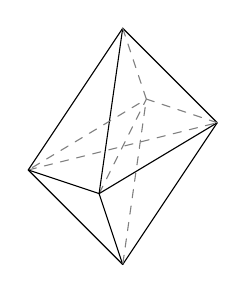
\begin{tikzpicture}[scale=1.5, line join=round, line cap=round]
      \coordinate (T) at (0,1);
      \coordinate (B) at (0,-1);
      \coordinate (E) at (0.8, 0.2);
      \coordinate (W) at (-0.8, -0.2);
      \coordinate (N) at (0.2, 0.4);
      \coordinate (S) at (-0.2, -0.4);
      
      \draw[dashed, gray] (W) -- (E);
      \draw[dashed, gray] (S) -- (N);
      
      \draw (T) -- (W) -- (B);
      \draw (T) -- (E) -- (B);
      \draw (T) -- (S) -- (B);
      \draw[dashed, gray] (T) -- (N) -- (B);
      
      \draw (W) -- (S) -- (E);
      \draw[dashed, gray] (E) -- (N) -- (W);
    \end{tikzpicture}
  \end{center}
\end{parts}

\vfill\rule{\linewidth}{0.4pt}

\begin{center}\small
\href{https://bhu-exam.vercel.app/}{Click here to visit our website}\\[4pt]
\href{https://me-aryan.vercel.app/}{Click here to visit our contributor}\\[4pt]
\href{https://quashan-me.vercel.app/}{Click here to visit our contributor}
\end{center}
\end{document}
